%--------------------------------------------------------------------------------
\documentclass[]{YIC2015}

% --------------------------------------------------------------------------------
% Include here your latex packages
%--------------------------------------------------------------------------------
\usepackage{graphicx}

% --------------------------------------------------------------------------------
% Article's title, with capital letter only at the beginning
%--------------------------------------------------------------------------------
\title{How to prepare a proceedings paper for YIC GACM 2015}

% -------------------------------------------------------------------------------
% List of authors
% --------------------------------------------------------------------------------
% Put the initials and surname of the first author ('et al.' if applicable) in
% square brackets before the command \author
%
% Identify the corresponding author with the command \corref and each author
% with the command \authref{a,b,...} according to the affiliation
%
\author[F. Author et al.]{F. Author\authref{a}\corref, S. Author\authref{a}, T.
Author\authref{b} }

% --------------------------------------------------------------------------------
% Affiliations
% --------------------------------------------------------------------------------
\address{\authaddr{a}{First Affiliation \\ %
	Address of the First Affiliation}
	\authaddr{b}{Second Affiliation \\ %
	Address of the Second Affiliation}
}
%
% --------------------------------------------------------------------------------
% Email address of the corresponding author
% --------------------------------------------------------------------------------
\corauth{corresponding.author@email.com}

% --------------------------------------------------------------------------------
% Abstract
% --------------------------------------------------------------------------------
\abstract{\textit{
Enter your abstract here (5 lines maximum). This document provides instructions for authors who write a proceedings paper for the YIC GACM 2015 Conference. A LaTeX class file and MS Word examples following the present format are available on the conference website. Papers should be converted into a pdf-file and both the Word/LaTeX file and the pdf file have to be uploaded before May 15th, 2015. To submit, go to the website http://registration.yic.rwth-aachen.de and upload the two files in the submission area (register if you have not already done so).
}}

% --------------------------------------------------------------------------------
% Keywords - must be separated by semicolon and no capital letters.
% --------------------------------------------------------------------------------
\keywords{The number of keywords is free, but should not exceed one line.}

% --------------------------------------------------------------------------------
% Beginning of document
% --------------------------------------------------------------------------------
\begin{document}

\maketitle

% --------------------------------------------------------------------------------
% Beginning of one section
% --------------------------------------------------------------------------------
\section{Introduction}
%
The members of the Scientific Committee will review the proceedings paper. For the paper to be included into the conference proceedings, it is mandatory that the abstract has been accepted to the conference and the conference fee has been paid before May 15th, 2015. Please note that only one proceedings paper per registered author is allowed.

\subsection{Proceedings Paper Format}
The total length of the proceedings paper (including figures, acknowledgements, references etc.) is 2 to 4 pages. The paper must be written in English.
The standard font type is Times (New) Roman for all titles and text.
The typing area is defined in %both Word
and LaTeX files. %Please, do not change the area.
This document should be used as a model for writing the text.

\section{Formatting details}

\subsection{Frontmatter Format}

The paper title must be left justified, using a 14pt size bold font. Use single line spacing and do not exceed three lines. The spacing before and after the title is 40pt and 8pt, respectively.

Authors and affiliations must be listed under the title. Type the name of the authors starting with their initials. If authors have different affiliations, group them together and use superscripts (a, b, c, \ldots). The names of the authors must be left justified, using a 12pt size regular font. The spacing after the authors is 16pt.
The affiliations must be left justified, using a 8pt size regular font and single line spacing. The affiliation must contain the name of the institute, department and the postal address. For each affiliation, add 6pt line spacing.

The e-mail address of the corresponding author must be left justified, using a 8pt size regular font. The spacing before and after the corresponding author e-mail address is 6pt and 34pt, respectively.

The abstract starts with the word `Abstract.' in 10pt bold font. The remaining text must use 10-point italic font. Type a short abstract of the paper (5 lines maximum). It must be written in one paragraph.  The abstract is not an introduction to the subject but a summary of the paper. It must explain the objectives, the tools and the conclusions. The spacing after the abstract is 12pt.

The keywords start with the word `Keywords:' in 10pt bold font. The number of key words is free, but do not exceed one line (typically, mention 3 to 6 keywords or groups of key words). Keywords must be typed using 10pt normal font. After the key words, leave 24pt vertical space before the main text.

\subsection{Main Text Format}

Primary headings are typed in 12pt bold capital letters, preceded by Arabic numbers (1, 2, 3, \ldots). They are left justified. Leave 12pt vertical space before and 6pt after primary headings.

Secondary headings are typed in 10pt bold letters, preceded by Arabic numbers (1.1, 1.2, 1.3, \ldots).  They are left justified.  Leave a 10pt vertical space before and a 5pt vertical space after secondary headings.

Tertiary headings are typed in 10pt bold letters, preceded by Arabic numbers (1.1.1, 1.1.2, 1.1.3, \ldots).  They are left justified. Leave a 6pt vertical space before tertiary headings and a 4pt vertical space after tertiary headings.

The main text is written using 10pt size regular font with single line spacing. Paragraphs must be left and right justified and not indented. Vertical space between paragraphs is stretchable to align contents on a page.

\subsubsection{Figures}
Figures must be numbered and captioned below. The caption is centered, in 10pt regular font. The spacing before the figure and after the caption is 10pt.

\begin{figure}[htbp]
\centering %
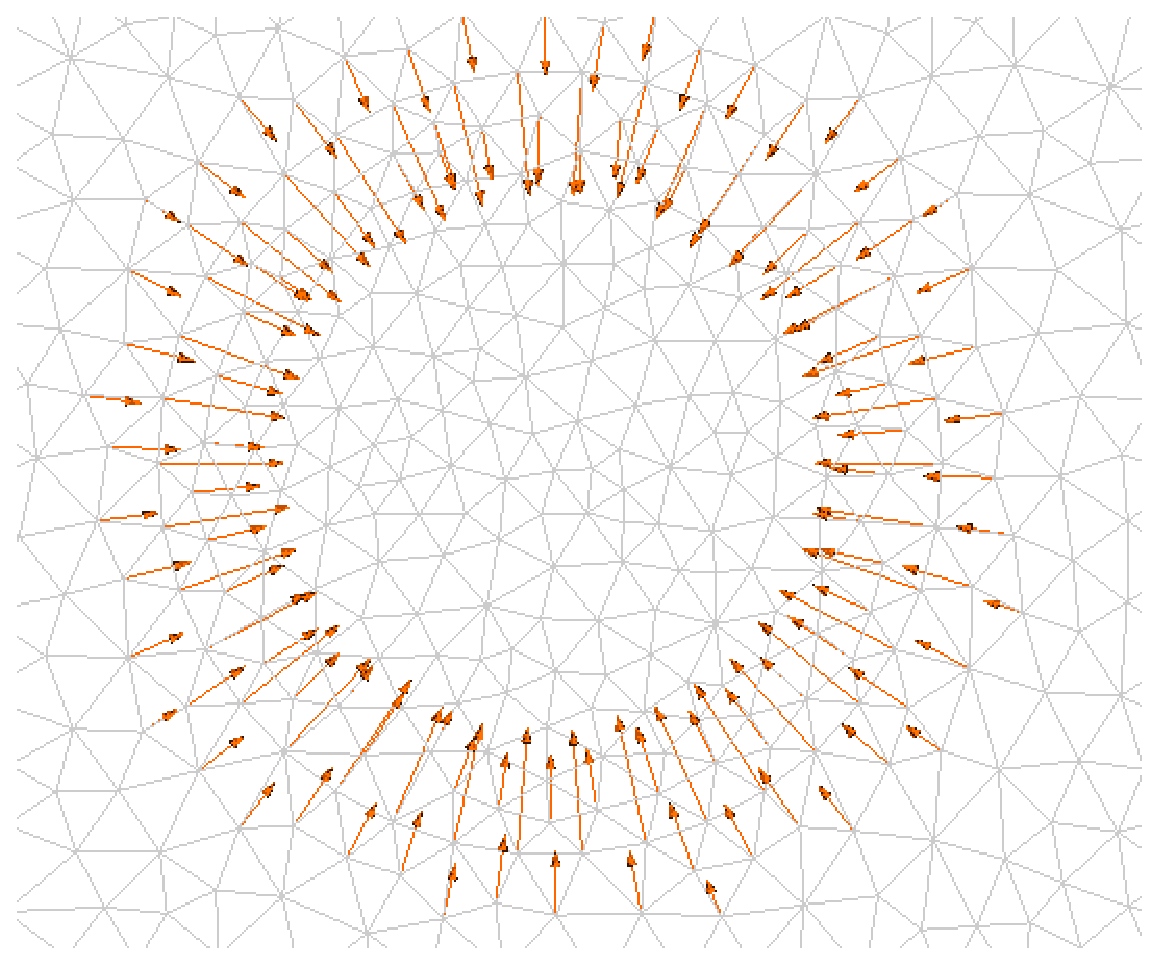
\includegraphics[width=50mm]{figure1.eps}
\caption{Figure caption.}
\label{fig:figure-manel1}
\end{figure}

Refer to figures in the text using the whole word, for example the model is shown in Figure \ref{fig:figure-manel1}. Make sure that legends in figures are of appropriate size.
%

\subsubsection{Tables}
\label{sec:Tables}
Table captions must be specified above the table. All tables must be numbered.
Use 10pt regular font for the caption and for the table itself. The spacing before and after the table is 10pt. Use borders to clearly separate the title row from the rest. See for example Table \ref{tab:table-silva1} in Section \ref{sec:Tables}.

%--------------------------------------------------------------------------------
% Example of a table.
%--------------------------------------------------------------------------------
\begin{table}[htdp]
\caption{Table caption.}
\centering
\begin{tabular}{lrrrl}
\hline\hline
\textbf{Subject} & \textbf{Value 1} & \textbf{Value 2} & \textbf{Value 3} & \textbf{Units} \\ \hline
Stress   &   123 & 23  & 45  &  MPa \\
Strain   &   123 & 23  & 45  &  --  \\
Pressure &   123 & 23  & 45  &  Pa  \\
Density  &   123 & 23  & 45  &  kg cm$^{-3}$ \\ \hline\hline
\end{tabular}
\label{tab:table-silva1}
\end{table}

\subsubsection{Equations}
Equations are centered and numbered between parentheses on the right of the line. Refer in the text to the equation using this number placed between parentheses, see for example Equation~(\ref{eq:hooke}) below:

\begin{equation}
\label{eq:hooke}
   \sigma_{11} = \frac{E}{(1+\nu)(1-2\nu)}
                 \left[(1-\nu)\varepsilon_{11}+\nu\varepsilon_{22}\right]
\end{equation}
\\
where $\sigma$ is the stress, $\varepsilon$ is the strain, $E$ is the Young's modulus and $\nu$ is the Poisson's coefficient. Small equations without reference can be put in the text directly, like $a = c/d$, but equations causing line stretching, like $\displaystyle a=\frac{c}{d}$, should be avoided. In that case a separate equation should be added, with or without number.

\subsection{References Format}
The bibliography should be the last section of the paper and use the layout as given in this example and 9pt font. Use an unnumbered heading `References' in the primary heading format. For a book reference use example~\cite{bookref}.  For a journal article use~\cite{articleref}. An article in proceedings should look like~\cite{procref}. The references should be labeled in the order in which they appear in the text. Place references in the text using a number or a list of numbers between square brackets.

\section{CONCLUSIONS}
Conclusions should briefly state the author's viewpoint over the problem and the most important propositions. They can also include the perspectives for new developments as well as for new applications from the results.

\section*{ACKNOWLEDGEMENTS}
Enter acknowledgements directly before the references. Use the format of primary section headers, but do not number the acknowledgement and references sections.


% --------------------------------------------------------------------------------
% Bibliography
% --------------------------------------------------------------------------------
\begin{thebibliography}{99}

% -------------------------------------------------------------------------------
% Bibliography - example of book's reference
% -------------------------------------------------------------------------------
\bibitem{bookref} %
F.~Author, S.~Author, T.~Author. \textit{Title}. Publisher, Year.

% --------------------------------------------------------------------------------
% Bibliography - example of journal's reference
% --------------------------------------------------------------------------------
\bibitem{articleref} %
F.~Author, S.~Author, T.~Author. Title. \textit{Journal Title} %
\textbf{Vol}:Pages, Year.

% --------------------------------------------------------------------------------
% Bibliography - example of proceedings' reference
% --------------------------------------------------------------------------------
\bibitem{procref}
F.~Author, S.~Author, T.~Author. Title. In: \textit{Proceedings Title}, City, Country, Day Month Year.

% --------------------------------------------------------------------------------
% Bibliography - the end.
% --------------------------------------------------------------------------------

\end{thebibliography}

% --------------------------------------------------------------------------------
% End of document
% --------------------------------------------------------------------------------
\end{document}
